%% =============================================================================
%% 快照（只读归档），不是当前投稿源。
%% 从 5090 还原：2026-08-21 18:23 +0800（昨晚）。
%% 当前正文仍是 main_wsdm2027_v3_zh.tex（2026-08-22 00:19）。
%% =============================================================================
% !TEX program = xelatex
% ============================================================
% 中文对照稿（阅读用，非投稿）
% 对应英文终稿：main_wsdm2027_v3.tex（2026-08-21 晚，0821zhidao derisk）
% 章节 / 图表 / 标签与英文稿一一对应，便于对照。
% Overleaf：Menu → Compiler → XeLaTeX
% ============================================================
\documentclass[sigconf,natbib=true,anonymous]{acmart}
%% WSDM 2027 — 中文对照 2026-08-20
%% 主表 GTS-Last/Random：cutoff-fit, no-cross
%% tab:early：等 horizon Early v2；tab:loov：GTS-Last warm
%% 变体名 TF / TF+LLM / TF+MV；tab:shift/tab:bucket = 全目标目录背景，不直接解释 warm MRR
%% app:intersection：Last∩Random 交集用户

\settopmatter{printacmref=false}
\renewcommand\footnotetextcopyrightpermission[1]{}
\setcopyright{none}
\acmConference[WSDM'27]{Proceedings of the 20th ACM International Conference on Web Search and Data Mining}{February 15--19, 2027}{Hong Kong}
\acmYear{2027}
\acmDOI{}
\acmISBN{}

\usepackage{booktabs}
\usepackage{multirow}
\usepackage{amsmath}
\let\Bbbk\relax
\usepackage{amssymb}
\usepackage{graphicx}
\usepackage{subcaption}
\usepackage{siunitx}
\usepackage{xspace}
\usepackage{enumitem}
\usepackage{microtype}
\usepackage{balance}
\usepackage{hyperref}

% XeLaTeX 中文（Overleaf 预装 Noto CJK）
\let\eth\relax
\usepackage{fontspec}
\usepackage{xeCJK}
\setCJKmainfont{Noto Serif CJK SC}
\setCJKsansfont{Noto Sans CJK SC}
\setCJKmonofont{Noto Sans Mono CJK SC}

\newcommand{\tfidf}{\textsc{TF-IDF}\xspace}
\newcommand{\llm}{\textsc{LLM}\xspace}
\newcommand{\tfllm}{\textsc{TF+LLM}\xspace}
\newcommand{\tfmv}{\textsc{TF+MV}\xspace}
\newcommand{\base}{\textsc{SASRec}\xspace}

\begin{document}

\title{更多文本视图有用吗？\\
面向序列推荐的泄漏感知文本表征评估}

\author{Anonymous Author(s)}
\affiliation{%
  \institution{Anonymous Institution}
  \country{}}
\renewcommand{\shortauthors}{Anonymous}

%==============================================================================
\begin{abstract}
%==============================================================================
%% 三条发现与提交稿一致；仅变体名统一为 TF / TF+LLM / TF+MV。
文本特征被广泛用于增强序列推荐，但对词法 \tfidf 与以 TF 为基座的 LLM 增量（单视图 \tfllm 或多提示视图 \tfmv）的比较，往往在允许时间重叠的评估协议下进行。
我们对仅 ID、截断拟合 \tfidf、\tfllm（在 \tfidf 基座上增加一个 Qwen2.5-7B 视图）以及 \tfmv（在 \tfidf 基座上增加四个提示视图）做泄漏感知对照实验，在三个 Amazon 数据集上采用全排序全局时间分割（GTS），以 GTS-Last 为主协议，GTS-Random 为稳健性检查，干净留一法（LOO）为对照。
得到三点发现。
第一，评估协议会改变结论：在所评估设置下，文本在热目标上一致优于仅 ID，但 \tfidf、\tfllm 与 \tfmv 的相对排序在 Last、Random 与 LOO 之间会变化——即使 Last 与 Random 评估的是同一组已训练检查点。
第二，没有任何文本表征能在不同时间窗口上稳健占优；时间偏移降低绝对性能，同时保持各文本变体之间的近平局。
第三，额外提示视图的边际收益有限，因为它们高度冗余：视图间 CKA 达 $0.82$--$0.94$，拼接表征仅使用名义有效秩的 $53$--$55\%$，留一视图对下游几乎无影响。
相比之下，TF-IDF 与 LLM 视图在几何上明显不同（CKA $\approx 0.19$），暗示存在词法--语义互补轴，而单纯增加提示视图并不能捕获这一轴。
这些结果表明，在把增益归因于越来越复杂的 LLM 文本管线之前，应先诊断评估协议与表征冗余。
\end{abstract}

\begin{CCSXML}
<ccs2012>
 <concept>
  <concept_id>10002951.10003317.10003347.10003350</concept_id>
  <concept_desc>Information systems~Recommender systems</concept_desc>
  <concept_significance>500</concept_significance>
 </concept>
 <concept>
  <concept_id>10002951.10003317.10003318.10003319</concept_id>
  <concept_desc>Information systems~Content ranking</concept_desc>
  <concept_significance>300</concept_significance>
 </concept>
</ccs2012>
\end{CCSXML}
\ccsdesc[500]{Information systems~Recommender systems}
\ccsdesc[300]{Information systems~Content ranking}

\keywords{序列推荐, 文本特征, 时间评估, 多视图冗余, 泄漏感知协议}

\maketitle

%==============================================================================
\section{引言}
\label{sec:intro}
%==============================================================================

序列推荐根据历史交互预测用户的下一个物品~\cite{kang2018sasrec,sun2019bert4rec,hidasi2016gru4rec}。
物品文本——标题、描述以及 LLM 生成的语义——是丰富 ID 嵌入并实现跨域迁移的标准手段~\cite{hou2022unisrec,bao2023tallrec}。
一个自然的工作假设是\emph{更丰富的文本总是更好}：LLM 嵌入应优于词袋，多个基于提示的视图应优于单视图。

这一假设被广泛持有。
近期工作表明，预训练语言表征可以改进文本增强推荐与可迁移性~\cite{hou2022unisrec,li2023recformer,bao2023tallrec}，特征级注意力可利用物品属性与文本~\cite{zhang2019fdsa}，多视图提示策略也越来越多地被用来捕捉功能、受众、风格等互补侧面。
构建生产推荐系统的从业者面临一个具体选择：是否应投入 LLM 推理与多提示管线来获取文本特征，还是轻量词袋基线已经足够？
答案高度依赖于比较是如何被评估的——这一考量在文本增强推荐论文中很少被审视。

该假设建立在脆弱的评估基础上。
大多数文本增强序列推荐器用留一法（LOO）分割来验证；如 \citet{ji2023evaluation} 与 \citet{sun2023reevaluation} 所示，LOO 允许训练与测试之间的时间重叠，从而抬高绝对指标，并可能扭曲模型比较。
在部署场景中，推荐器必须预测用户\emph{将来}会交互的物品，而不是重建一个随机持出的历史交互。
全局时间分割（GTS）更好地模拟这一部署约束，但也引入额外设计选择：\emph{目标选择模式}（每位用户在测试窗口内取 Last、Random、Successive 或 All）本身会改变有效任务难度，并可能改变模型排名~\cite{gusak2025time}。
已有工作一般性地研究了分割效应~\cite{meng2020temporal,ji2023evaluation}；我们表明这些效应对 \tfidf vs.\ \tfllm vs.\ \tfmv 的比较\emph{尤为决定性}。

文本特征还需要预处理——词汇构建、IDF 加权、SVD 投影以及 LLM 嵌入白化——每一步都必须尊重时间边界。
若这些统计量在完整物品集（含未来物品）上计算，所得特征会携带训练时不可用的信息，引入一种与训练/测试分割正交的泄漏。
因此我们全程强制严格的\emph{截断拟合}：所有文本预处理仅在训练截断之前出现的物品上拟合。

我们比较五种变体——ID、\tfidf、\tfllm、\tfmv，以及改编的 UniSRec 基线~\cite{hou2022unisrec}——在三个 Amazon 数据集上，协议为 GTS-Last（主）、GTS-Random（稳健性检查）与干净 LOO（对照），外加等 horizon 的 Early 时间窗口。
变体按完整特征组成命名：基于 \llm 的变体是对词法 \tfidf 基座的\emph{增量}，而非替换；不含基座的纯 LLM 变体在第~\ref{sec:discussion}~节单独评估。
我们用 CKA~\cite{kornblith2019cka}、有效秩~\cite{roy2007effective} 与留一视图（LOOV）诊断多视图行为。

\smallskip\noindent\textbf{研究问题。}
\begin{enumerate}[leftmargin=*,itemsep=1pt]
\item[\textbf{RQ1}] \emph{协议效应。}
干净 LOO、GTS-Last 与 GTS-Random 是否改变 \tfidf、\tfllm 与 \tfmv 的绝对增益与相对排序？
\item[\textbf{RQ2}] \emph{时间稳健性。}
Main 时间窗口（$80\%$ 截断）下的结论，在训练窗口缩小（Early，$60\%$ 截断）后是否仍然成立？
\item[\textbf{RQ3}] \emph{多视图冗余。}
为何四个提示视图（\tfmv）不能可靠地优于单视图（\tfllm）甚至单独的 \tfidf，潜在互补性在哪里？
\end{enumerate}

\smallskip\noindent\textbf{贡献。}
\begin{enumerate}[leftmargin=*,itemsep=1pt]
\item 在三个数据集上的泄漏感知比较表明，评估协议会改变文本表征的排序。在 GTS 内部，同一组已训练检查点上的 Last vs.\ Random 会产生不同赢家（\textbf{目标效应}）；从 GTS 切到 LOO 则同时改变训练数据与目标（\textbf{分割效应}）。文本一致优于 ID，但\emph{哪种}文本最好是协议敏感的。
\item 跨窗口证据表明没有单一文本变体占优：在匹配协议的 Early 窗口（前 $60\%$ 训练、随后 $10\%$ 验证、再随后 $10\%$ 测试；最后 $20\%$ 不用）下，绝对 MRR 下降，Main 窗口的排序不被保持，但各文本变体彼此仍相差不超过 0.001。
\item 三角验证的冗余分析（CKA + 有效秩 + LOOV），覆盖原始 3584 维 Qwen 隐状态直至 64 维白化后表征，共同刻画了有限的多视图增益，并识别词法--语义不相似性（TF vs.\ LLM，CKA $0.18$--$0.20$）作为潜在互补轴。
\end{enumerate}

%==============================================================================
\section{相关工作}
\label{sec:related}
%==============================================================================

\paragraph{文本增强序列推荐。}
早期系统将词袋或评论文本与协同过滤融合~\cite{wang2015cdl,salton1988termweighting}。
现代方法用预训练语言模型编码标题与描述，以支持跨域迁移~\cite{hou2022unisrec,hou2023vqrec,geng2022p5,bao2023tallrec}。
UniSRec 从文本学习可迁移物品表征，并用轻量 MoE 适配~\cite{hou2022unisrec}；VQ-Rec 量化文本嵌入以支持迁移~\cite{hou2023vqrec}；P5 将推荐写成语言建模~\cite{geng2022p5}；TALLRec 通过指令微调把 LLM 对齐到排序~\cite{bao2023tallrec}。
这些系统通常报告 LOO 或定义不严的时间协议。
我们\emph{不}提出新架构；我们问的是：在固定骨干、控制时间泄漏之后，更强的文本编码器与更多视图是否仍然有优势。

\paragraph{基于 LLM 的物品表征。}
在架构论文之外，一种日益常见的做法是把 LLM 嵌入当作即插即用的物品特征——可以是单视图（标题/描述），也可以是多个提示条件视图，据称能捕捉互补侧面（功能、受众、风格）。
其动机是：不同提示可以引出物品的不同语义方面（例如「描述功能」vs.\「描述目标受众」），从而扩大特征覆盖。
然而，当所有视图都由\emph{同一个}预训练编码器作用于\emph{同一段}物品文本时，所得表征的多样性取决于编码器内部表征对指令变化的实际响应程度——这一问题在推荐文献中几乎没有实证关注。
本研究把这一表征选择从架构创新中隔离出来：固定同一 SASRec 骨干与融合管线，只改变文本来源（单独 \tfidf、\tfllm 或 \tfmv）。

\paragraph{评估协议与时间泄漏。}
采样指标会扭曲排序~\cite{krichene2020sampledmetrics}；LOO 与基于时间的分割会改变绝对分数，并可能改变模型选择~\cite{ji2023evaluation,sun2023reevaluation,meng2020temporal}。
\citet{hidasi2018recurrent} 表明，看似细微的协议选择就能造成序列模型相对排序的大幅变化。
在 GTS 内部，目标选择模式也很重要：\citet{gusak2025time} 表明 Successive 最接近在线下一物品预测但代价高；Last 是确定性低成本代理；Random 与 Successive 的秩相关最高（因 Random 非确定性，我们对三个采样种子取平均）；All 把多个物品打进同一真值集合，引入任务不匹配，且与 Successive 相关最弱。
在序列推荐之外，时间协议的影响也已在会话推荐~\cite{hidasi2018recurrent} 与一般协同过滤~\cite{meng2020temporal} 中得到记录，说明协议敏感性不是局部问题，而是跨推荐范式的系统性关切。
我们将这一发现专门化到文本表征：协议会改变结论，\emph{正是因为} \tfidf、\tfllm 与 \tfmv 对分布偏移的响应不同。
验证与测试的目标模式对齐（同为 Last，或同为 Random）也被建议用于可靠的模型选择~\cite{gusak2025time}；我们的 Early 窗口实验保持这一对齐。

\paragraph{多视图学习与表征冗余。}
多视图理论认为视图必须\emph{有用且互补}；更多视图并不保证收益~\cite{xu2013multiview}。
在计算机视觉中，\citet{kornblith2019cka} 引入 CKA（Centered Kernel Alignment）来衡量跨网络层与架构的 Gram 结构相似性；即使实例级两两余弦中等或接近零，CKA 仍能检测结构冗余。
在 NLP 中，\citet{ethayarajh2019contextual} 揭示同一预训练模型不同层的上下文词嵌入高度各向异性，占据嵌入空间中的窄锥，这是一种几何冗余。
有效秩（归一化奇异值的熵）~\cite{roy2007effective} 提供互补诊断，量化名义维度中有多少被实际使用。
这些工具已被用于分析网络深度~\cite{kornblith2019cka} 与嵌入质量~\cite{ethayarajh2019contextual}，但据我们所知，尚未被联合用于诊断推荐中的\emph{多提示}冗余。
我们结合 CKA、有效秩与 LOOV——而不是任何单一指标——来解释有限的多视图增益。

\paragraph{嵌入的信息几何。}
奇异值集中与各向异性是预训练文本嵌入的已知失效模式~\cite{ethayarajh2019contextual}。
当多个视图由同一编码器生成时，这些几何性质会传播：每个视图继承相似的谱结构，拼接并不会按比例扩张有效子空间。
我们的有效秩分析把这一文献连接到序列推荐：拼接四个共享同一编码器的提示视图得到 ER/dim $\approx$0.53，而同维度的词法 \tfidf SVD 保留 ER/dim $\approx$0.98。

%==============================================================================
\section{对照实验设置}
\label{sec:setup}
%==============================================================================

\subsection{时间协议}
\label{sec:protocol}

\paragraph{GTS-Last（主协议）。}
交互按时间戳全局排序。
\textbf{Main} 窗口使用 RecBole 的 \texttt{TS} 分割~\cite{zhao2021recbole} $[0.8,0.1,0.1]$：前 $80\%$ 交互用于训练，随后 $10\%$ 用于验证，最后 $10\%$ 用于测试。
序列增强之后，每位用户只贡献其\textbf{时间上最后一个}测试交互（每用户一个目标）——即 \citet{gusak2025time} 研究的确定性末项代理。

\paragraph{Early 窗口（RQ2）。}
Early 使用全局有序交互的前 $60\%$ 训练、随后 $10\%$ 验证、再随后 $10\%$ 测试；最后 $20\%$ 不用（RecBole \texttt{TS} $[0.6,0.1,0.1]$；三个分数不重新归一化到和为 1）。
评估窗口前移，而验证/测试 horizon 长度仍各固定为 $10\%$（与 Main 等 horizon）。

\paragraph{GTS-Random（稳健性检查）。}
同一组检查点；每位用户贡献一个\textbf{均匀随机}的测试交互。我们对三个目标采样种子（42、123、456）取平均以保证稳定；每个检查点的跨种子标准差为 0.001--0.003。
Random 与 Successive 的秩相关最高~\cite{gusak2025time}，用作交叉核对。

\paragraph{干净 LOO（对照）。}
按用户留一、无全局时间截断：对每位用户，除最后两次交互外全部用于训练，倒数第二次用于验证，最后一次用于测试（RecBole \texttt{LS} 分割）。
仅用于量化协议差距；\emph{不}用于主结论。

\paragraph{GTS-All（附录）。}
每位用户的全部截断后目标；因任务不匹配~\cite{gusak2025time} 放入附录~\ref{app:gts-all}。

\paragraph{泄漏控制。}
\tfidf 词汇/IDF、SVD 投影以及 LLM 中心化/白化，仅在训练截断前出现的物品上拟合。
评估过滤训练交互 $\ge 5$ 的用户。
主表报告\textbf{热目标}结果：测试目标必须属于训练期物品目录，该目录同时也是推理时的候选集。
Last 与 Random 在每个数据集上评估\emph{同一合格用户集合}（通过 min-5 过滤且在测试窗口有交互：Beauty 4{,}520，Toys 4{,}873，Grocery 4{,}152）；两种模式的差别只在于选取哪一次目标交互。
由于热过滤作用于\emph{被选中的}目标，两种模式的热子队列略有差别（例如 Beauty：Last 下 3{,}137 名热用户，Random 各采样种子为 3{,}054--3{,}083）。
为确认这一二阶差异不驱动我们的结论，附录~\ref{app:intersection} 将两种模式限制到其热队列的交集（在 Last \emph{且} Random 下均为热的用户）：在每个数据集、两种模式下方法排序均不变，因此 Last vs.\ Random 的对比是固定用户群体上的目标选择效应。
全目标与未见物品诊断见附录~\ref{app:alltarget}。

\subsection{文本表征与模型}
\label{sec:models}

所有变体共享 \base~\cite{kang2018sasrec} 骨干（$d{=}256$，2 层，2 个注意力头）。

\begin{itemize}[leftmargin=*,itemsep=1pt]
\item \textbf{ID}：仅 ID 嵌入。
\item \textbf{TF}：训练截断 \tfidf $\to$ SVD 256 维 $\to$ 轻量投影头 + InfoNCE 对齐~\cite{oord2018cpc}。
\item \textbf{\tfllm}：TF 的 \tfidf 基座\emph{加上}单个 Qwen2.5-7B~\cite{qwen2024qwen25} 物品嵌入（训练截断中心化与白化）；两种来源由同一管线融合。
\item \textbf{\tfmv}：\tfidf 基座\emph{加上}四个提示视图（Description / Function / Audience / Style）$\to$ 每视图 64 维投影 $\to$ 256 维拼接 $\to$ 共享投影；无交叉注意力。
\item \textbf{UniSRec}~\cite{hou2022unisrec}：原始 UniSRec 架构（物品文本嵌入上的 MoE 适配器）在各数据集上从头训练、无跨域预训练；为泄漏对等，其物品文本输入替换为同一套截断拟合、白化后的 Qwen2.5-7B 嵌入，并使用相同评估过滤。因此我们将其视为\emph{适配到我们截断拟合特征的 UniSRec 骨干}，而非原始预训练 UniSRec。
\end{itemize}

变体名称把特征组成写清楚：基于 LLM 的变体是对词法基座的\emph{增量}而非替换，因此 RQ1 比较的是固定 \tfidf 基座上的增量增强，而不是三个独立表征家族。
不含基座的纯 LLM 变体在第~\ref{sec:discussion}~节评估。
所有文本变体采用两阶段训练：Phase~A（经 InfoNCE 预热文本头），然后 Phase~B（联合 BPR~\cite{rendle2009bpr} + InfoNCE 微调）。
超参数、融合（无交叉、无 boost）以及 Early 窗口的截断拟合预处理均从 Main 冻结（不重调）；评估窗口前移，而验证/测试 horizon 长度保持固定。

\subsection{数据集}

Amazon Beauty、Toys \& Games 与 Grocery \& Gourmet Food~\cite{mcauley2015amazon,ni2019amazon}：
\begin{itemize}[leftmargin=*,itemsep=1pt]
\item \textbf{Beauty}：121 万用户，25.9 万物品，202 万交互。
\item \textbf{Toys}：128 万用户，33.6 万物品，225 万交互。
\item \textbf{Grocery}：76.8 万用户，17.2 万物品，130 万交互（同平台复现；不宣称领域多样性）。
\end{itemize}

\subsection{评估细节}

全排序 Hit@10、NDCG@10、MRR@10~\cite{krichene2020sampledmetrics}。
主表：MRR@10，3 个训练种子（42、2024、2026）的均值$\pm$样本标准差；NDCG/Hit 作为次要指标。
全部运行在单张 NVIDIA RTX 5090 上；每模型训练 15--65~分钟。

%==============================================================================
\section{RQ1：协议改变排序}
\label{sec:rq1}
%==============================================================================

\begin{table}[t]
\centering
\caption{%
协议对照——热目标 MRR@10（3 个训练种子均值$\pm$标准差，min5 过滤；GTS-Random 另外对 3 个目标采样种子取平均）。
\textbf{加粗}：每行在基于 \base 的变体（ID / TF / TF+LLM / TF+MV）中的最佳。
UniSRec 为适配后的外部基线，在 Grocery 上最强。
赢家随协议变化（点估计；图~\ref{fig:protocol} 中 1 个标准差内的差距用 $\approx$）：Last 偏向 \tfmv；Random 使 TF 与 \tfmv 持平；LOO 偏向 \tfllm$\approx$\tfmv$\approx$TF。%
}
\label{tab:protocol}
\small
\setlength{\tabcolsep}{2.2pt}
\begin{tabular}{@{}llccccc@{}}
\toprule
数据集 & 协议 & ID & TF & TF+LLM & TF+MV & UniSRec \\
\midrule
\multirow{3}{*}{Beauty}
 & GTS-Last  & .0032\tiny{$\pm$.0006} & .0053\tiny{$\pm$.0004} & .0060\tiny{$\pm$.0004} & \textbf{.0064}\tiny{$\pm$.0003} & .0052\tiny{$\pm$.0002} \\
 & GTS-Rand  & .0074\tiny{$\pm$.0005} & \textbf{.0124}\tiny{$\pm$.0002} & .0120\tiny{$\pm$.0002} & \textbf{.0124}\tiny{$\pm$.0002} & .0096\tiny{$\pm$.0001} \\
 & LOO       & .0175\tiny{$\pm$.0004} & .0251\tiny{$\pm$.0002} & \textbf{.0254}\tiny{$\pm$.0004} & .0253\tiny{$\pm$.0004} & .0239\tiny{$\pm$.0002} \\
\midrule
\multirow{3}{*}{Toys}
 & GTS-Last  & .0031\tiny{$\pm$.0002} & .0040\tiny{$\pm$.0005} & .0035\tiny{$\pm$.0002} & \textbf{.0042}\tiny{$\pm$.0006} & .0040\tiny{$\pm$.0008} \\
 & GTS-Rand  & .0076\tiny{$\pm$.0002} & \textbf{.0113}\tiny{$\pm$.0004} & .0108\tiny{$\pm$.0007} & .0108\tiny{$\pm$.0009} & .0085\tiny{$\pm$.0003} \\
 & LOO       & .0152\tiny{$\pm$.0005} & .0247\tiny{$\pm$.0006} & .0258\tiny{$\pm$.0012} & \textbf{.0258}\tiny{$\pm$.0028} & .0196\tiny{$\pm$.0010} \\
\midrule
\multirow{2}{*}{Grocery}
 & GTS-Last  & .0030\tiny{$\pm$.0012} & .0046\tiny{$\pm$.0006} & .0047\tiny{$\pm$.0005} & \textbf{.0058}\tiny{$\pm$.0007} & .0107\tiny{$\pm$.0002} \\
 & GTS-Rand  & .0050\tiny{$\pm$.0012} & .0087\tiny{$\pm$.0011} & .0076\tiny{$\pm$.0004} & \textbf{.0089}\tiny{$\pm$.0008} & .0121\tiny{$\pm$.0002} \\
\bottomrule
\end{tabular}
\end{table}

\begin{figure}[t]
\centering
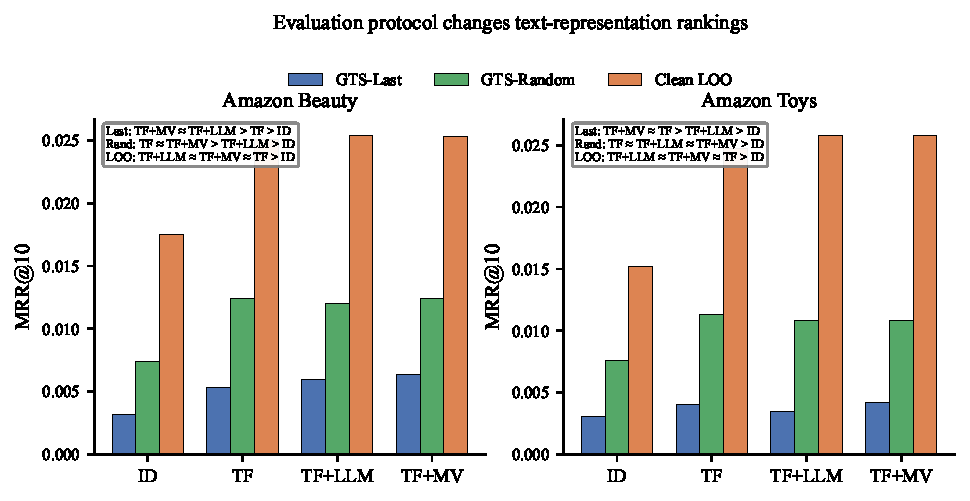
\includegraphics[width=\linewidth]{figures/fig_protocol_contrast.pdf}
\caption{%
Beauty 与 Toys 上的协议对照。
柱为 3 种子\emph{点估计}（GTS-Last/Random：热 MRR@10；Random 再对 3 个目标采样种子取平均；LOO：干净留一，仅作对照）。
图内排序在差距落在 1 个种子级标准差内时用 $\approx$，不是唯一冠军声称。
Last vs.\ Random 会改变基于 \base 的文本变体中的排序；LOO 抬高绝对值，三种文本方法近并列。%
}
\label{fig:protocol}
\end{figure}

\begin{table}[t]
\centering
\caption{%
GTS-Last 热 NDCG@10 与 Hit@10（3 种子均值$\pm$标准差）。
在基于 \base 的变体中，NDCG 与 MRR 一致。
UniSRec 在 Hit@10（三个数据集）以及 Grocery 的 NDCG 上最强。%
}
\label{tab:ndcg_hit}
\small
\setlength{\tabcolsep}{2.5pt}
\begin{tabular}{@{}llccccc@{}}
\toprule
数据集 & 指标 & ID & TF & TF+LLM & TF+MV & UniSRec \\
\midrule
\multirow{2}{*}{Beauty}
 & NDCG & .0047\tiny{$\pm$.0007} & .0074\tiny{$\pm$.0006} & .0080\tiny{$\pm$.0009} & \textbf{.0087}\tiny{$\pm$.0003} & .0081\tiny{$\pm$.0003} \\
 & Hit  & .0098\tiny{$\pm$.0013} & .0146\tiny{$\pm$.0013} & .0146\tiny{$\pm$.0029} & .0167\tiny{$\pm$.0011} & \textbf{.0180}\tiny{$\pm$.0007} \\
\midrule
\multirow{2}{*}{Toys}
 & NDCG & .0046\tiny{$\pm$.0004} & .0056\tiny{$\pm$.0006} & .0046\tiny{$\pm$.0002} & .0057\tiny{$\pm$.0011} & \textbf{.0066}\tiny{$\pm$.0013} \\
 & Hit  & .0098\tiny{$\pm$.0013} & .0108\tiny{$\pm$.0011} & .0084\tiny{$\pm$.0004} & .0108\tiny{$\pm$.0027} & \textbf{.0154}\tiny{$\pm$.0030} \\
\midrule
\multirow{2}{*}{Grocery}
 & NDCG & .0048\tiny{$\pm$.0019} & .0062\tiny{$\pm$.0004} & .0063\tiny{$\pm$.0005} & .0077\tiny{$\pm$.0007} & \textbf{.0160}\tiny{$\pm$.0003} \\
 & Hit  & .0107\tiny{$\pm$.0041} & .0117\tiny{$\pm$.0009} & .0117\tiny{$\pm$.0007} & .0136\tiny{$\pm$.0007} & \textbf{.0338}\tiny{$\pm$.0007} \\
\bottomrule
\end{tabular}
\end{table}

\begin{table}[t]
\centering
\caption{%
分种子 GTS-Last 热 MRR@10（种子 42 / 2024 / 2026）。
方差可见；\tfmv 的领先幅度小，且依赖种子。%
}
\label{tab:perseed}
\small
\setlength{\tabcolsep}{3pt}
\begin{tabular}{@{}llccccc@{}}
\toprule
数据集 & 种子 & ID & TF & TF+LLM & TF+MV & UniSRec \\
\midrule
\multirow{3}{*}{Beauty}
 & 42    & .0038 & .0049 & .0063 & .0063 & .0050 \\
 & 2024  & .0032 & .0052 & .0055 & .0066 & .0054 \\
 & 2026  & .0026 & .0057 & .0063 & .0061 & .0051 \\
\midrule
\multirow{3}{*}{Toys}
 & 42    & .0033 & .0045 & .0037 & .0035 & .0044 \\
 & 2024  & .0030 & .0038 & .0032 & .0042 & .0045 \\
 & 2026  & .0029 & .0036 & .0036 & .0048 & .0031 \\
\bottomrule
\end{tabular}
\end{table}

表~\ref{tab:protocol} 与图~\ref{fig:protocol} 报告协议对照。
没有任何文本表征处处获胜；相对排序随目标选择协议而变：

\begin{itemize}[leftmargin=*,itemsep=1pt]
\item \textbf{GTS-Last}：在受控的基于 \base 的变体中，\tfmv 在三个数据集上都是点估计领先者（Beauty $.0064$，Toys $.0042$，Grocery $.0058$），但若干差距在 1 个标准差内（Toys：\tfmv$\approx$TF；表~\ref{tab:perseed}）；改编的 UniSRec 基线在 Grocery 上最强（$.0107$）。
\item \textbf{GTS-Random}（3 个采样种子平均）：TF 在 Toys 上为点估计领先（$.0113$ vs.\ \tfmv $.0108$，在 1 个标准差内）；Beauty 打平（TF $.0124$，\tfmv $.0124$）；Grocery 上 \tfmv 领先 $.0002$（$.0089$ vs.\ $.0087$），远在 1 个标准差内。
\item \textbf{LOO}：绝对 MRR 比 GTS-Last 高 4--7 倍；三种文本方法近并列（\tfllm $\approx$ \tfmv $\approx$ TF）。
\end{itemize}
Last vs.\ Random 是同一组已训练 GTS 检查点上的\textbf{目标选择}效应；LOO vs.\ GTS 是\textbf{分割/训练协议}效应（不同的训练数据与模型）。

\paragraph{对 LOO 差距的一种合理解释。}
LOO 下 4--7 倍更高的绝对分数不只是加性平移；它也改变了文本方法之间的相对排序。
LOO 允许时间重叠：用户的训练交互包含与测试目标同一时期的物品，使模型能够「记忆」在严格时间截断下本不存在的共现模式。
一种合理解释是：这种重叠不成比例地有利于捕捉细粒度语义相似的表征（\tfllm 与 \tfmv），因为重叠物品为语义特征提供的共现信号比词法特征更丰富。
在 GTS 下，训练与评估\emph{交互}被全局时间截断分开，这一优势不再可用，\tfidf 更宽的词法覆盖变得有竞争力。
（热评估仍要求目标物品属于训练目录，因此物品集合在时间上并非不相交。）

\paragraph{为何 Last 与 Random 不一致？}
Last 与 Random 在同一组已训练检查点、同一合格用户上评分，差别只在选取哪一次测试交互；排序翻转在相交热用户上仍然成立（附录~\ref{app:intersection}）。
这就是目标选择效应~\cite{gusak2025time}。
一种合理解释是：Last 与 Random 从测试窗口抽出不同的物品流行度混合，因此在一种混合下排序更高的表征不必在另一种下也更高。
我们没有直接统计表明 Last 目标偏向最近流行、趋势或小众物品，也不声称词法 vs.\ 语义的因果机制。

\paragraph{含义。}
\emph{同一组检查点}（同一训练权重），在同一合格用户上评估，当目标选择从 Last 换成 Random 时会产生不同赢家——这是目标选择带来的协议伪影。
因此，若不指定目标模式，文本表征优越性的声称并不可靠。
在我们评估的每一种协议下，所有文本方法都优于仅 ID（GTS-Last 下相对 $+$13--100\%，Random 下差距更大）。
数据因此支持窄声称（文本优于 ID），而不支持宽声称（存在单一最佳文本表征）。

\paragraph{UniSRec 作为外部基线。}
在相同的 GTS-Last + min5 + 热过滤下，UniSRec 得分为 $0.0052$（Beauty）与 $0.0040$（Toys），在 Beauty 上介于 ID 与 TF 之间、在 Toys 上与 TF 持平，但在 Grocery 上占优（$0.0107$，接近次优的 2 倍）。
表~\ref{tab:ndcg_hit} 表明，GTS-Last 下 NDCG@10 大体与 MRR 排序一致，而 Hit@10 在三个数据集上都抬高 UniSRec，因此指标选择与协议相互作用。
我们因此以 MRR 作为主排序指标，并报告 NDCG/Hit 以供完整。
UniSRec 的表观排序对协议敏感：去掉 min5 过滤后，GTS-Last 的 MRR 会抬到 0.02 量级（附录~\ref{app:unisrec}）。
最小交互阈值、候选范围（热 vs.\ 全）以及目标模式，各自都能独立改变外部基线的表观排序。

%==============================================================================
\section{RQ2：时间稳健性}
\label{sec:rq2}
%==============================================================================

\begin{table}[t]
\centering
\caption{%
Beauty 上 Main（前 $80\%$ 训练、随后 $10\%$ 验证、最后 $10\%$ 测试）vs.\ Early（前 $60\%$ 训练、随后 $10\%$ 验证、再随后 $10\%$ 测试；最后 $20\%$ 不用）——GTS-Last 热 MRR@10（3 种子均值$\pm$标准差）。
融合与截断拟合嵌入与 Main 对齐；超参数冻结。
Main 行与表~\ref{tab:protocol} 一致。
点估计：Main 上 \tfmv 最高；Early 上 \tfidf 最高（与 \tfmv 在 1 个标准差内）。%
}
\label{tab:early}
\small
\begin{tabular}{@{}lccc@{}}
\toprule
窗口 & TF & TF+LLM & TF+MV \\
\midrule
Main      & .0053\tiny{$\pm$.0004} & .0060\tiny{$\pm$.0004} & \textbf{.0064}\tiny{$\pm$.0003} \\
Early60-EQ & \textbf{.0042}\tiny{$\pm$.0005} & .0037\tiny{$\pm$.0003} & .0039\tiny{$\pm$.0003} \\
\bottomrule
\end{tabular}
\end{table}

\begin{table}[t]
\centering
\caption{%
全目标目录级背景（valid$\to$test，Main GTS），\emph{不是}对热目标 MRR 的直接解释。
未见目标不在训练目录中，从不进入表~\ref{tab:protocol} 与~\ref{tab:early} 的热分数。
报告为与目录偏移的关联，而非因果声称。%
}
\label{tab:shift}
\small
\setlength{\tabcolsep}{4pt}
\begin{tabular}{@{}lccc@{}}
\toprule
数据集 & 未见目标 & 流行度均值（V$\to$T） & 流行度中位数（V$\to$T） \\
\midrule
Beauty  & 31.9\% & $112.8 \to 101.8$ & $21 \to 15$ \\
Toys    & 40.8\% & $144.7 \to 119.1$ & $18 \to 11$ \\
Grocery & 29.6\% & $87.3 \to 76.9$ & $16 \to 12$ \\
\bottomrule
\end{tabular}
\end{table}

\begin{table}[t]
\centering
\caption{%
全目标流行度分桶构成（valid$\to$test，Main GTS；head $\ge$10，mid 3--9，low 1--2 次训练交互）。
仅作目录级背景：未见物品被热过滤排除，不进入热 MRR。%
}
\label{tab:bucket}
\small
\setlength{\tabcolsep}{3.5pt}
\begin{tabular}{@{}llcccc@{}}
\toprule
数据集 & 分割 & Head & Mid & Low & Unseen \\
\midrule
\multirow{2}{*}{Beauty}
 & Valid & 63.1\% & 15.9\% & 9.7\% & 11.3\% \\
 & Test  & 56.6\% & 14.9\% & 10.7\% & 17.8\% \\
\midrule
\multirow{2}{*}{Toys}
 & Valid & 60.1\% & 16.3\% & 10.6\% & 13.0\% \\
 & Test  & 52.3\% & 15.5\% & 11.0\% & 21.3\% \\
\bottomrule
\end{tabular}
\end{table}

为把训练窗口大小的效应从测试 horizon 长度中隔离出来，我们使用等 horizon 的 Early 分割：前 $60\%$ 交互训练、随后 $10\%$ 验证、再随后 $10\%$ 测试；最后 $20\%$ 不用（RecBole \texttt{TS} $[0.6,0.1,0.1]$）。
评估窗口前移，而验证/测试 horizon 长度仍各固定为与 Main 相同的 $10\%$。

表~\ref{tab:early} 报告两个窗口在相同无交叉、无 boost、截断拟合协议下的 GTS-Last 热 MRR@10。
从 Main 到 Early，每个变体的绝对分数都下降。
窗口内排序\emph{不是}不变的：点估计在 Main 上偏向 \tfmv，在 Early 上偏向 \tfidf（$.0042$ vs.\ \tfmv $.0039$ 与 \tfllm $.0037$，与 \tfmv 在 1 个标准差内）。
三者彼此仍相差不超过 $0.001$。
因此 Main 窗口「\tfmv 略领先」的模式并不能作为时间事实成立。
表~\ref{tab:early} 中的 Main$\to$Early 下降只在热目标上测量。
表~\ref{tab:shift}--\ref{tab:bucket} 提供同一全局截断下的全目标\emph{目录级背景}（未见占比、流行度）；它们不是对热 MRR 下降的直接解释，因为未见物品从不进入这些分数（附录~\ref{app:alltarget}）。

一旦时间窗口变化，就没有单一文本变体占优。

\paragraph{把偏移连接到表征类型。}
我们没有按物品的统计表明 TF-IDF 在物品间均匀退化，也没有表明 Last 目标由流行物品主导。
一种合理解释——与表~\ref{tab:early} 中 \tfidf 的 Main$\to$Early 下降小于 \tfllm/\tfmv 相一致——是：当评估窗口前移时，词法特征与 LLM 增量特征的响应不同。
我们强调关联而非因果：目录级偏移统计与 Main$\to$Early 下降共现，但我们不声称未见占比或流行度偏移\emph{导致}热目标上的排序模式。

%==============================================================================
\section{RQ3：为何多视图增益有限}
\label{sec:rq3}
%==============================================================================

\begin{figure}[t]
\centering
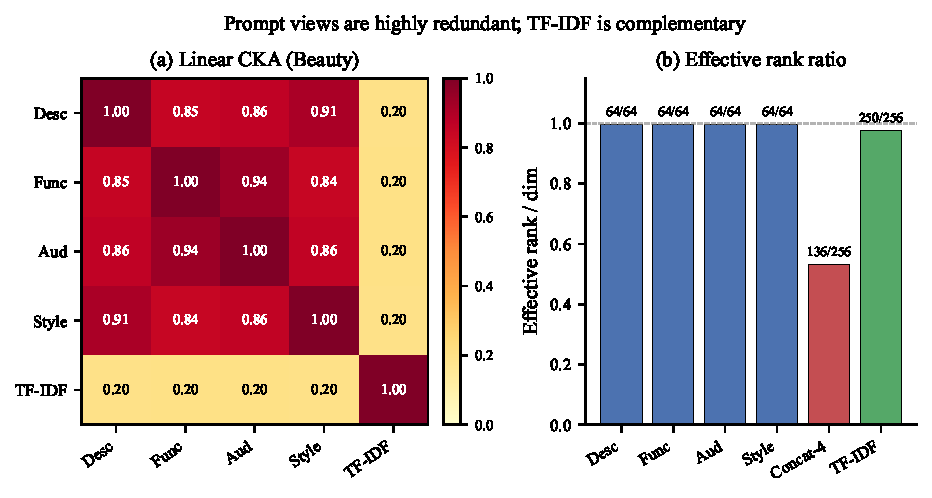
\includegraphics[width=\linewidth]{figures/fig_cka_heatmap.pdf}
\caption{%
Beauty 上的表征分析（3 次随机抽取各 3{,}000 个物品，均值$\pm$标准差）。
\textbf{(a)}~成对 CKA：LLM 视图彼此高度相似（0.84--0.94）；TF--LLM CKA 较低（$\approx$0.20）。
\textbf{(b)}~有效秩：4 视图拼接 136/256（53\%），TF-IDF 为 250/256（98\%）。%
}
\label{fig:cka}
\end{figure}

\begin{table}[t]
\centering
\caption{%
视图间 CKA（3 次各 3K 物品子样本，均值$\pm$标准差）。
所有 LLM 视图对均超过 0.82；TF-IDF 与任一 LLM 视图保持在 0.18--0.20。%
}
\label{tab:cka}
\small
\setlength{\tabcolsep}{4pt}
\begin{tabular}{@{}lcc@{}}
\toprule
视图对 & Beauty & Toys \\
\midrule
Description--Function  & $.846 \pm .001$ & $.834 \pm .001$ \\
Description--Audience  & $.860 \pm .001$ & $.856 \pm .002$ \\
Description--Style     & $.914 \pm .000$ & $.904 \pm .001$ \\
Function--Audience     & $.940 \pm .000$ & $.921 \pm .001$ \\
Function--Style        & $.843 \pm .001$ & $.818 \pm .002$ \\
Audience--Style        & $.859 \pm .001$ & $.838 \pm .002$ \\
\midrule
\emph{TF-IDF vs.\ LLM 视图（范围）} & $.196$--$.201$ & $.184$--$.189$ \\
\bottomrule
\end{tabular}
\end{table}

\begin{table}[t]
\centering
\caption{%
有效秩（Beauty/Toys，3 次子样本）。
4 视图拼接只占据名义维度的 53--55\%。%
}
\label{tab:effrank}
\small
\begin{tabular}{@{}lccc@{}}
\toprule
表征 & 维数 & ER（Beauty） & ER（Toys） \\
\midrule
单 LLM 视图（平均） & 64 & 63.7 (99.5\%) & 63.6 (99.4\%) \\
4 视图拼接 & 256 & 136.1 (\textbf{53.2\%}) & 141.2 (\textbf{55.2\%}) \\
TF-IDF（SVD） & 256 & 249.9 (97.6\%) & 251.4 (98.2\%) \\
\bottomrule
\end{tabular}
\end{table}

\begin{table}[t]
\centering
\caption{%
留一视图（零掩码，3 种子均值），协议为 GTS-Last 热，与表~\ref{tab:protocol} 对齐。
$\Delta$：相对完整 4 视图模型的热 MRR@10 变化。
最大 $|\Delta|$ 为 0.00032（Beauty 上的 Style）。%
}
\label{tab:loov}
\small
\setlength{\tabcolsep}{3.5pt}
\begin{tabular}{@{}lccccc@{}}
\toprule
数据集 & Full MRR & $-$Desc & $-$Func & $-$Aud & $-$Style \\
\midrule
Beauty & .00636 & $-$.00021 & $-$.00030 & $-$.00027 & $-$.00032 \\
Toys   & .00417 & $-$.00017 & $+$.00005 & $-$.00007 & $-$.00025 \\
\bottomrule
\end{tabular}
\end{table}

我们用三项互补分析回答 RQ3，单独任何一项都不够：CKA 捕捉结构相似性，但本身不能证明任务无关~\cite{kornblith2019cka}；有效秩衡量维度利用率；LOOV 衡量下游影响。

\paragraph{（1）高视图间 CKA。}
表~\ref{tab:cka} 与图~\ref{fig:cka}(a) 表明，全部六对 LLM 视图的 CKA $\ge 0.82$（Beauty 0.84--0.94；Toys 0.82--0.92）。
四个提示视图由同一编码器作用于同一物品文本、仅指令不同，编码了高度相似的关系结构。
相比之下，TF-IDF 与任一 LLM 视图的 CKA 为 0.196--0.201（Beauty）与 0.184--0.189（Toys）——这是质上不同的区间，表明表征明显不相似。

\paragraph{（2）成对余弦 vs.\ CKA。}
提示视图之间的平均成对余弦常常中等或接近零（例如 Beauty 上 Description--Function $\approx -0.01$），而 Function--Audience 可达 $\approx 0.42$。
这\emph{并不}与高 CKA 矛盾：余弦衡量向量的实例级对齐，CKA 比较整个物品集上的 Gram 矩阵几何~\cite{kornblith2019cka}。
视图可以平均余弦很低，却仍诱导近乎同构的相似结构——这正是我们在基于提示的释义上观察到的区间。
因此我们把 CKA 作为主相似性诊断，余弦只作互补核对，从不单独当作冗余证明。

\paragraph{（3）拼接视图的低有效秩。}
表~\ref{tab:effrank} 与图~\ref{fig:cka}(b) 表明，把四个 64 维视图拼成 256 维，有效秩仅为 136（Beauty）与 141（Toys），只占据可用容量的 53--55\%。
近一半名义维度携带冗余结构。
同为 256 维的 TF-IDF 有效秩 $\ge$250（97--98\%），几乎用满容量。
因此拼接提示视图对子空间的扩张，远小于维数表面所暗示的。

\paragraph{（4）可忽略的 LOOV 影响。}
表~\ref{tab:loov} 表明，在 GTS-Last 热下将任一单视图置零，下游影响极小：最大 $|\Delta|$ = 0.00032（约为完整 \tfmv 分数的 5\%）。
完整 MRR 与表~\ref{tab:protocol} 的 \tfmv 列一致。
分种子符号可能翻转，因此我们不把任何提示视为不可或缺。

\paragraph{冗余从何而来？}
为把提示诱导的冗余与预处理诱导的冗余分开，我们比较两个阶段的 CKA：\emph{白化前}（SVD 投影 + 中心化，每视图 64 维，\textbf{不做} ZCA 白化）与\emph{白化后}（最终模型输入嵌入）。
在 Beauty 上，平均成对 CKA 白化前为 $0.96\pm0.001$，白化后为 $0.88\pm0.001$；Toys 上分别为 $0.96\pm0.001$ 与 $0.87\pm0.001$。
CKA 在\emph{白化之前就已经极高}（表~\ref{tab:cka-prepost}）：白化把平均视图间 CKA 降低 0.08（Beauty）与 0.10（Toys），并把拼接有效秩从 Beauty 的 99/256（39\%）提高到 136/256（53\%），Toys 从 104/256 提高到 140/256。

为把冗余追溯得更靠前，我们直接在\emph{任何 SVD 投影之前}的原始 3584 维 Qwen 隐状态上计算视图间 CKA。
3584 维上的平均成对 CKA 在 Beauty 为 $0.961$，Toys 为 $0.963$（3 次随机抽取 3000 物品，$\sigma < 0.002$）。
拼接 4 视图矩阵（$4\times 3584 = 14336$ 维）的有效秩在 Beauty 仅为 1567（10.9\%），Toys 为 1622（11.3\%）。
因此，在我们的提示设计下，冗余在 SVD 或白化之前就已经存在于原始 Qwen 输出中，而非 SVD 截断的伪影：四种指令变体在 3584 维上诱导近乎同构的关系结构，$\sim$90\% 的维度塌缩在该阶段已经存在。
这一审计无法把编码器内在塌缩、与使用同一物品文本、或提示不够发散区分开来。
白化部分去相关了视图，但不能消除这一结构重叠。
因此把视图维度扩到 $4\times256$ \emph{并不}合理——瓶颈是该提示设计下的源头冗余，不是投影容量（表~\ref{tab:cost}）。

\begin{table}[t]
\centering
\caption{%
白化前 vs.\ 白化后审计（3 次物品子样本，均值）。
CKA 在白化前已 $\ge$0.94；白化降低 CKA 并提高拼接有效秩，因此冗余不是白化伪影。
子样本独立于表~\ref{tab:effrank} 抽取，故 Toys 白化后秩有 $\pm 1$ 的差别。%
}
\label{tab:cka-prepost}
\small
\begin{tabular}{@{}llcc@{}}
\toprule
数据集 & 阶段 & 成对 CKA & 拼接 ER/256 \\
\midrule
\multirow{2}{*}{Beauty}
 & 白化前（SVD+中心化）  & 0.94--0.99 & 99 (39\%) \\
 & 白化后（TS 拟合）     & 0.84--0.94 & 136 (53\%) \\
\midrule
\multirow{2}{*}{Toys}
 & 白化前（SVD+中心化）  & 0.94--0.98 & 104 (41\%) \\
 & 白化后（TS 拟合）     & 0.82--0.92 & 140 (55\%) \\
\bottomrule
\end{tabular}
\end{table}

\paragraph{综合。}
三项诊断一致：提示视图编码重叠语义，导致维度塌缩与可忽略的单视图贡献。
观测到的几何与多视图理论意义上的视图互补不足相一致~\cite{xu2013multiview}（由单一来源经语义释义得到的视图）。
我们系统中的潜在互补性在词法 \tfidf 与语义 \llm 视图之间（CKA $0.18$--$0.20$），表明朴素多提示堆叠并未收获这种表征不相似性：\tfmv 模型把相似语义结构复制了四次，而不是进一步利用它已经包含的词法--语义轴。

%==============================================================================
\section{讨论与局限}
\label{sec:discussion}
%==============================================================================

\paragraph{为何单独 TF-IDF 能与 \tfmv 持平？}
为何词袋表征能在 GTS-Random 下匹配甚至超过四视图变体？
我们看到两个因素。
第一，\tfidf 捕捉\emph{词法多样性}：产品标题与描述的词汇覆盖数万独特 token，SVD 投影后的 TF-IDF 几乎保留全部可用容量（ER/dim $\approx$0.98；表~\ref{tab:effrank}）。
每个维度贡献不同信息。
第二，四个 LLM 视图受\emph{语义同质}之苦：同一预训练编码器处理同一物品文本，仅指令略有变化，所得表征共享高度相似的关系几何（CKA 0.82--0.94）。
拼接四个这样的视图在名义上把维度扩到四倍，但实际只增加约 $50\%$ 新容量。
TF-IDF 并不比 LLM 捕捉更丰富的语义，但其\emph{每维几何多样性}高得多。
这种每维几何多样性在 GTS-Random 下成为实践优势：热目标上 \tfidf 与 \tfmv 持平或更好（表~\ref{tab:protocol}），尽管拼接后的 LLM 视图只占用约一半名义秩（表~\ref{tab:effrank}）。

\paragraph{纯 LLM（无 \tfidf 基座）消融。}
因为 \tfllm 与 \tfmv 是对 \tfidf 基座的增量，人们会问 LLM 视图单独能做到多少。
我们训练一个只用单个 Qwen2.5-7B 视图、\emph{没有} \tfidf 基座的变体（相同架构、相同两阶段管线）。
在主协议（GTS-Last 热，min5，训练目录候选）下，该纯 LLM 变体在 Beauty 上为 $.0046\pm.0001$，Toys 上为 $.0018\pm.0007$——低于表~\ref{tab:protocol} 的 \tfllm 列（$.0060$ / $.0035$），并在 Toys 上低于仅 ID。
因此词法基座是承重的，不是「免费初始化」：我们所有文本增益都是锚定于 \tfidf 的管线增益，这也是我们把变体命名为 \tfllm 与 \tfmv，而不是 LLM 与 MV 的原因。

\paragraph{单视图混合：丢掉四个视图中的三个。}
为检验 RQ3 识别的词法--语义不相似性（TF--LLM CKA $0.18$--$0.20$）是否承载有用信号，我们训练一个混合体：保留 \tfidf 基座，并在多视图架构内只保留\emph{一个} LLM 视图（每视图投影 + 拼接；无额外提示视图），协议与训练种子与表~\ref{tab:protocol} 相同（截断拟合、无交叉）。
在 GTS-Last 热下，混合体为 $.0070\pm.0006$（Beauty）与 $.0049\pm.0011$（Toys），对比 \tfmv 的 $.0064\pm.0003$ / $.0042\pm.0006$；在 GTS-Random（3 个采样种子）下为 $.0128\pm.0003$ 与 $.0114\pm.0008$，对比 \tfmv 的 $.0124\pm.0002$ / $.0108\pm.0009$。
因此混合体在两个数据集、两种目标模式下匹配或略超四视图模型，同时只用一个而非四个提示视图；优势大约在 1 个种子级标准差内，我们将其读作\emph{丢掉三个视图并无损失}外加一贯的小优势，而不是大幅加性增益。
这与冗余分析相一致：额外提示视图在单视图之外贡献很少，有用信号由词法--语义对承载。
低 TF--LLM CKA 本身只许可\emph{几何不相似}；混合体提供了排序层面的证据。

\paragraph{对从业者的含义。}
\begin{enumerate}[leftmargin=*,itemsep=2pt]
\item 在 GTS 下报告文本表征比较，并明确目标模式。LOO 可能翻转排序，并给出 4--7 倍更高的绝对指标。
\item 以截断拟合 \tfidf 作为强基线起步。在 GTS-Random 下，它在三个数据集上都与 \tfmv 相差不超过 1 个标准差，并在 Toys 上领先；在 Main 窗口的 GTS-Last 下它可能落后于 \tfllm/\tfmv，但表~\ref{tab:early} 表明更早截断可以翻转该排序。相对 LLM 推理，其预处理成本可忽略，因此 TF-IDF 应是首先评估的文本基线。
\item 单个 \llm 视图通常与四个提示视图持平；在投入多视图管线之前，先用 CKA 与有效秩等诊断冗余。
\item 从同一编码器增加更多提示视图，收益可忽略。表征家族之间的几何多样性（词法 \tfidf vs.\ 语义 \llm）才是更有用的轴：在我们的实验中，\tfidf + 单 LLM 视图混合体在 GTS-Last 与 GTS-Random 下都匹配或略超 \tfmv。此类声称应在 GTS-Last/Random 下验证，而不能从低 CKA 或 GTS-All 验证分数直接假定。
\item 不要跨协议过度声称单一「最佳」文本表征；把 Last 与 Random（或 Successive）并列报告，因为排序可能在目标模式之间翻转。
\end{enumerate}

\paragraph{局限。}
\begin{itemize}[leftmargin=*,itemsep=1pt]
\item \textbf{热目标范围。}
我们的模型没有仅内容的零样本回退；热目标评估因此是最公平的比较，但它排除了 28--35\% 合格用户的末项测试目标（以及 30--41\% 的全部截断后目标）。
\item \textbf{静态元数据。}
我们使用固定的产品标题/描述；随时间演化的文本（如评论、趋势标签）可能改变 TF/LLM 平衡。
\item \textbf{仅 Amazon 领域。}
三个数据集都是 Amazon 子类。Grocery 是同平台复现，不是领域多样性的解决方案。
\item \textbf{GTS-Random 可复现性。}
我们对三个目标采样种子（42、123、456）平均 GTS-Random。每个检查点热 MRR@10 的跨种子标准差为 0.001--0.003，表明对目标采样有中等但不可忽略的敏感性~\cite{gusak2025time}。
\item \textbf{冗余位点。}
我们的冗余审计现覆盖三个阶段——原始 3584 维 Qwen 隐状态、256 维 SVD 投影、64 维白化后——表明在我们的提示设计下，冗余在 SVD/白化之前就已经存在于原始 Qwen 输出中（第~\ref{sec:rq3}~节）。该设计无法把编码器内在塌缩与共享物品文本或提示不够发散区分开来。只测试了一个 LLM（Qwen2.5-7B）；其他架构可能呈现不同的视图间结构。
\item \textbf{Successive 未完整运行。}
我们依赖 Last/Random 作为代理；在抽样用户上做 Successive 健全性检查将进一步验证协议选择。
\end{itemize}

\paragraph{成本分析。}
\begin{table}[t]
\centering
\caption{推荐阶段参数量与在线打分成本（种子~42；\emph{不含离线文本编码}）。\tfmv 增加 $<$1\% 参数。}
\label{tab:cost}
\small
\begin{tabular}{@{}lcc@{}}
\toprule
模型 & 参数（M） & ms/样本 \\
\midrule
ID / TF / TF+LLM / TF+MV & 67.2 / 67.4 / 67.6 / 67.7 & 0.02 \\
UniSRec & 67.7 & 0.04 \\
\bottomrule
\multicolumn{3}{@{}l}{\footnotesize Beauty；Toys 因词表更大约为 87M（排序相同）。}
\end{tabular}
\end{table}

表~\ref{tab:cost} 确认多视图失败不是容量问题：所有变体的推荐阶段参数预算与在线打分成本实质上相同。
实践成本差距在\emph{离线文本编码}，表中有意排除：截断拟合 \tfidf+SVD 在 Beauty 目录（25.9 万物品，实测）上大约只需一分钟 CPU，而每个 Qwen2.5-7B 视图需要对目录做一次一次性 GPU 推理，多视图把该遍数乘以提示数。
特征侧成本、而非模型侧成本，才是 \tfidf、\tfllm 与 \tfmv 的差别所在。

%==============================================================================
\section{结论}
\label{sec:conclusion}
%==============================================================================

我们对序列推荐的文本表征做了泄漏感知对照实验，定位为实证研究而非新模型论文。
实验给出三点结论。

\begin{enumerate}[leftmargin=*,itemsep=1pt]
\item \textbf{协议很重要。}
\tfidf、\tfllm 与 \tfmv 的相对排序依赖于 GTS 目标模式。
文本特征一致优于仅 ID，但哪种文本最好需要指定评估协议。
在基于 \base 的变体中，\tfmv 在 GTS-Last 下于三个数据集上为点估计领先（改编的 UniSRec 基线在 Grocery 上最强）；在 GTS-Random 下，\tfidf 追上并在 Toys 上反超，差距不超过 1 个标准差。这一变化完全由目标选择驱动，而非模型变化。
\item \textbf{没有文本变体一贯占优。}
在匹配协议的 Early 窗口（前 $60\%$ 训练、随后 $10\%$ 验证、再随后 $10\%$ 测试；最后 $20\%$ 不用）下，绝对 MRR 下降，Main 排序不被保持（\tfidf 最高，差距在 1 个标准差内），但各文本变体彼此仍相差不超过 0.001。
文本有帮助，但哪种文本帮助最大，既取决于表征，也同样取决于评估窗口。
\item \textbf{多视图增益受视图间冗余限制。}
CKA、有效秩与 LOOV 共同表明提示视图编码重叠语义；潜在互补性在词法与语义特征之间（CKA $0.18$--$0.20$），而不在同一编码器上的不同提示指令之间。
与此一致，保留 \tfidf 基座与单个 LLM 视图的混合体在 GTS-Last 与 GTS-Random 下都匹配或略超 \tfmv（第~\ref{sec:discussion}~节）：提示视图预算更应花在词法--语义对上，而不是额外提示上。
\end{enumerate}

文本增强序列推荐越来越被当作 LLM 升级问题——更多参数、更多提示、更多视图被假定会单调提升质量。
我们的证据表明，社区应先锁定时间协议，再诊断表征冗余，然后再投入额外提示视图或融合模块。
泄漏感知评估下的实践默认是：报告 GTS-Last（并以 Random 作核对），把截断拟合 \tfidf 作为强制基线，并把多视图 LLM 特征当作有待检验的假说——而不是免费升级。

\paragraph{未来方向。}
五个问题仍开放。
(1)~\textbf{更丰富的词法--语义融合。} 我们的单视图混合体在 GTS-Last/Random 下匹配或略超 \tfmv；更复杂的融合（如门控、交叉注意力）能否把词法--语义对变成更大、显著的增益，仍待检验。
(2)~\textbf{跨架构冗余审计。} 原始 3584 维审计表明，观测到的冗余在我们的提示下已经存在于 Qwen2.5-7B 输出中。检验同一视图塌缩是否也出现在仅解码 vs.\ 仅编码 LLM（如 Mistral、BERT-large）上，将有助于把编码器家族与提示设计分开。
(3)~\textbf{GTS-Successive 评估}（抽样用户规模），以验证 Last/Random 作为在线下一物品预测代理~\cite{gusak2025time}。
(4)~\textbf{非 Amazon 领域}且时间戳可靠，以检验协议敏感性是否超出产品目录。
(5)~\textbf{指令多样化提示}，强制语义分歧（如属性抽取 vs.\ 情感摘要），以检验互补性能否在提示层被工程化。

\section*{伦理考量}
本工作使用公开 Amazon 评论数据集，除标准用户/物品 ID 外不含个人可识别属性。
潜在关切包括时间偏移下强化流行度偏差，以及继承 LLM 生成文本特征中的偏差。
我们通过报告热目标分层诊断缓解前者，并通过把多视图 LLM 特征当作经验研究对象而非推荐默认来缓解后者。
未涉及人类受试者。

\begin{acks}
匿名评审。
\end{acks}

%==============================================================================
\appendix
%==============================================================================

\section{GTS-All 结果}
\label{app:gts-all}

主表使用 GTS-Last（每用户一个末项目标）。
GTS-All 评估全部截断后目标（Beauty：4{,}520 用户 $\to$ 12{,}001 样本，人均 2.65；Toys：4{,}873 用户 $\to$ 13{,}186，人均 2.71）。

\begin{table}[h]
\centering
\caption{GTS-All 热 MRR@10（3 种子均值；所有列均为截断拟合检查点）。
在 All 下 TF 领先或与 \tfmv 打平，不同于 GTS-Last。}
\label{tab:gts-all}
\small
\begin{tabular}{@{}lccccc@{}}
\toprule
数据集 & ID & TF & TF+LLM & TF+MV & UniSRec \\
\midrule
Beauty & .0156 & \textbf{.0241} & .0237 & \textbf{.0241} & .0180 \\
Toys   & .0118 & \textbf{.0191} & .0180 & .0184 & .0139 \\
\bottomrule
\end{tabular}
\end{table}

在 GTS-All 下，TF 在两个数据集上都领先或与 \tfmv 打平，更接近 GTS-Random 而非 GTS-Last（后者 \tfmv 在基于 \base 的变体中略领先）。
按 \citet{gusak2025time}，All 与 Successive 的秩相关最低并引入任务不匹配，因此我们将其放入附录，不把这些排序当作主协议结果。

\section{Grocery 分种子明细}
\label{app:grocery}

\begin{table}[h]
\centering
\caption{Grocery 热 MRR@10，按训练种子，GTS-Last 与 GTS-Random（Random 对目标采样种子 $\{42,123,456\}$ 取平均）。}
\label{tab:grocery-perseed}
\small
\setlength{\tabcolsep}{3pt}
\begin{tabular}{@{}llcccc@{}}
\toprule
协议 & 种子 & ID & TF & TF+LLM & TF+MV \\
\midrule
\multirow{3}{*}{GTS-Last}
 & 42    & .0027 & .0038 & .0049 & .0052 \\
 & 2024  & .0019 & .0049 & .0050 & .0058 \\
 & 2026  & .0043 & .0050 & .0041 & .0065 \\
\midrule
\multirow{3}{*}{GTS-Rand}
 & 42    & .0044 & .0075 & .0073 & .0088 \\
 & 2024  & .0041 & .0095 & .0080 & .0082 \\
 & 2026  & .0063 & .0091 & .0075 & .0097 \\
\bottomrule
\end{tabular}
\end{table}

Grocery 在相同搜索预算下复现 Beauty/Toys 模式：在基于 \base 的变体中，Last 上 \tfmv 略领先，Random 上 TF 与 \tfmv 相差不超过 1 个标准差。
我们将其视为同平台复现，而非领域多样性声称。

\section{GTS-Random 目标采样种子}
\label{app:random-seeds}

主表 GTS-Random 数字是在同一组检查点上对三个目标采样种子 $\{42,123,456\}$ 取平均（不重训）。
表~\ref{tab:random-seeds} 报告每个采样种子在三个训练种子上的平均。
热 MRR@10 的跨种子标准差通常为 0.001--0.003；种子 456 系统性更低，因此单个 Random 种子会夸大 TF 在 Beauty 上的领先（0.0138 vs.\ 3 种子 0.0124）。

\begin{table}[h]
\centering
\caption{GTS-Random 热 MRR@10，按目标采样种子（训练种子 42/2024/2026 的均值）。}
\label{tab:random-seeds}
\small
\setlength{\tabcolsep}{3pt}
\begin{tabular}{@{}llccccc@{}}
\toprule
数据集 & 采样种子 & ID & TF & TF+LLM & TF+MV & UniSRec \\
\midrule
\multirow{3}{*}{Beauty}
 & 42    & .0081 & .0138 & .0133 & .0134 & .0098 \\
 & 123   & .0080 & .0134 & .0128 & .0141 & .0103 \\
 & 456   & .0063 & .0101 & .0099 & .0098 & .0087 \\
\midrule
\multirow{3}{*}{Toys}
 & 42    & .0096 & .0146 & .0140 & .0141 & .0103 \\
 & 123   & .0066 & .0091 & .0089 & .0085 & .0078 \\
 & 456   & .0065 & .0101 & .0095 & .0098 & .0075 \\
\bottomrule
\end{tabular}
\end{table}

\section{Last vs.\ Random：交集用户}
\label{app:intersection}

Last 与 Random 对同一合格用户计分，但热过滤作用于\emph{被选中的}目标，因此两个热子队列并不完全重合（第~\ref{sec:protocol}~节）。
原则上，Last vs.\ Random 的排序差异可能部分是队列构成伪影，而非纯目标选择效应。
我们通过在其热队列的\emph{交集}上重评两种模式来排除这一点——即 Last 目标\emph{与} Random 目标都落在训练目录中的用户——使用同一组检查点、每个检查点一次前向，使每用户排名与主表背后的排名相同。
交集保留 Beauty 2{,}846--2{,}858 用户（合格用户的 63\%）、Toys 2{,}651--2{,}686（54\%）、Grocery 2{,}671--2{,}678（64\%），仅随 Random 采样种子变化。

表~\ref{tab:intersection} 报告交集上的热 MRR@10，并并列主表~\ref{tab:protocol} 与~\ref{tab:ndcg_hit} 的完整热队列。
两点观察在全部六个数据集$\times$模式块中成立。
第一，限制到交集最多把绝对分数改变 $.0014$（最大在 Beauty Random：去掉仅 Last 为热的用户后，TF 从 $.0124$ 降到 $.0110$），且 ID、\tfidf、\tfllm 与 \tfmv 的排序不变。
第二，更重要的是，我们依赖的 Last$\to$Random 变化在同一用户集合上仍然成立：Last 下 \tfmv 在三个数据集上领先；Random 下 \tfidf 在 Beauty（$.0110$ vs.\ $.0113$）与 Grocery（$.0083$ vs.\ $.0087$）追到 1 个标准差内，并在 Toys 上反超 \tfmv（$.0110$ vs.\ $.0105$）。
对每个变体，Random 也大约仍是 Last 的两倍容易。
因此两种效应都可单独归因于目标选择。

\begin{table}[h]
\centering
\caption{交集用户（Last 与 Random 下均为热）上的热 MRR@10，对比主表完整热队列。3 个训练种子均值$\pm$标准差；Random 另外对目标采样种子 $\{42,123,456\}$ 取平均。}
\label{tab:intersection}
\small
\setlength{\tabcolsep}{3pt}
\begin{tabular}{@{}llcccc@{}}
\toprule
& & \multicolumn{2}{c}{Last} & \multicolumn{2}{c}{Random} \\
\cmidrule(lr){3-4}\cmidrule(lr){5-6}
数据集 & 变体 & 交集 & 完整热 & 交集 & 完整热 \\
\midrule
\multirow{4}{*}{Beauty}
 & ID     & .0033$\pm$.0006 & .0032$\pm$.0005 & .0066$\pm$.0004 & .0074$\pm$.0004 \\
 & \tfidf & .0054$\pm$.0003 & .0053$\pm$.0003 & .0110$\pm$.0002 & .0124$\pm$.0002 \\
 & \tfllm & .0063$\pm$.0004 & .0060$\pm$.0003 & .0107$\pm$.0003 & .0120$\pm$.0001 \\
 & \tfmv  & .0065$\pm$.0003 & .0064$\pm$.0002 & .0113$\pm$.0002 & .0124$\pm$.0002 \\
\midrule
\multirow{4}{*}{Toys}
 & ID     & .0032$\pm$.0001 & .0031$\pm$.0001 & .0073$\pm$.0001 & .0076$\pm$.0001 \\
 & \tfidf & .0039$\pm$.0005 & .0040$\pm$.0004 & .0110$\pm$.0003 & .0113$\pm$.0003 \\
 & \tfllm & .0035$\pm$.0002 & .0035$\pm$.0002 & .0106$\pm$.0005 & .0108$\pm$.0006 \\
 & \tfmv  & .0040$\pm$.0004 & .0042$\pm$.0005 & .0105$\pm$.0008 & .0108$\pm$.0008 \\
\midrule
\multirow{4}{*}{Grocery}
 & ID     & .0031$\pm$.0010 & .0030$\pm$.0010 & .0047$\pm$.0010 & .0050$\pm$.0010 \\
 & \tfidf & .0049$\pm$.0005 & .0046$\pm$.0005 & .0083$\pm$.0010 & .0087$\pm$.0009 \\
 & \tfllm & .0050$\pm$.0004 & .0047$\pm$.0004 & .0071$\pm$.0002 & .0076$\pm$.0003 \\
 & \tfmv  & .0063$\pm$.0005 & .0058$\pm$.0005 & .0087$\pm$.0007 & .0089$\pm$.0006 \\
\bottomrule
\end{tabular}
\end{table}

\section{全目标与交叉注意力}
\label{app:alltarget}

\paragraph{全目标评估。}
纳入未见测试物品（不在训练目录中）会均匀降低绝对 MRR，但保持排序。
全部测试目标中的未见占比：Beauty 31.9\%，Toys 40.8\%，Grocery 29.6\%。
这些目标从不进入主表的热目标分数；它们量化部署期流量中有多少被热评估排除，而不是热 MRR 为何下降（表~\ref{tab:shift}--\ref{tab:bucket} 是同一套全目标目录背景）。
没有仅内容的零样本能力时，所有模型在未见物品上接近零分；热目标范围是最公平的比较。

\paragraph{交叉注意力（负结果）。}
\label{app:cross}
测试过序列级交叉注意力模块（关注文本视图特征），但对每用户性能的提升与下降大致相当；因此排除在主方法之外。

\section{UniSRec 详细结果}
\label{app:unisrec}

UniSRec~\cite{hou2022unisrec} 对评估过滤高度敏感：没有 \texttt{min\_train\_inter}=5 过滤时，其 MRR@10 可达 0.0204--0.0208（Beauty）与 0.0162--0.0164（Toys）。
在共享协议（min5 过滤）下：

\begin{table}[h]
\centering
\small
\begin{tabular}{@{}lccc@{}}
\toprule
数据集 & GTS-All & GTS-Last & GTS-Random$^\dagger$ \\
\midrule
Beauty & .0180$\pm$.0001 & .0052$\pm$.0002 & .0096$\pm$.0001 \\
Toys   & .0139$\pm$.0003 & .0040$\pm$.0008 & .0085$\pm$.0003 \\
\bottomrule
\end{tabular}
\end{table}

\noindent$^\dagger$GTS-Random 对目标采样种子 $\{42,123,456\}$ 取平均（与表~\ref{tab:protocol} 相同协议）。
三列均为同一组截断拟合检查点上的热目标 MRR@10。

在公平比较下，UniSRec 在 Beauty MRR 上介于 ID 与 TF 之间，在 Toys 上与 TF 持平，这与它使用单个 LLM 视图、且没有使我们的 \tfllm/\tfmv 变体受益的对齐预热相一致。
在 GTS-Last 的 Hit@10 上 UniSRec 更强（表~\ref{tab:ndcg_hit}），说明骨干差异对不同指标的影响不同。

\bibliographystyle{ACM-Reference-Format}
\bibliography{refs}

\end{document}
